\documentclass[runningheads]{llncs}

\usepackage[T1]{fontenc}
\usepackage{amsmath,amssymb,amsfonts}
\usepackage{algorithmic}
\usepackage{graphicx}
\usepackage{xcolor}
\usepackage{booktabs}
\usepackage{url}
\usepackage{array}
\usepackage{multirow}
\usepackage{placeins}

\newcolumntype{L}[1]{>{\raggedright\arraybackslash}p{#1}}

\begin{document}

\title{A Drift-Aware MLOps Framework for Multi-Model Serving: A Network Intrusion Detection Case Study}

\titlerunning{A Drift-Aware MLOps Framework for Multi-Model Serving}

\author{Hoang Tran-Nguyen-Viet\inst{1} \and
Thai Bui-Ngoc\inst{1} \and
Tuan Le-Anh\inst{1} \and
Bao Nguyen-Van\inst{1} \and
Quan Le-Trung\inst{1}
}

\authorrunning{Hoang Tran-Nguyen-Viet et al.}

\institute{Faculty of Computer Networks and Communications,\\
University of Information Technology, VNU-HCM,\\Ho Chi Minh City, Vietnam\\
\email{\{23520541,23521412\}@gm.uit.edu.vn, \{tuanla,baonv,quanlt\}@uit.edu.vn}}

\maketitle

\begin{abstract}
Machine learning services can degrade when production data distributions change, even if source code remains unchanged. This issue is critical for network intrusion detection, where benign traffic and attack behavior evolve over time. This paper presents a baseline drift-aware MLOps framework for user-imported and training-job-created tabular models, using Network Intrusion Detection Systems (NIDS) as a case study rather than proposing a new classifier. The contributions are threefold: a tenant-aware control-plane/data-plane architecture in which a PostgreSQL-backed Native Registry owns product-level lifecycle state; a drift-aware formulation connecting onboarding, inference logs, reference and current windows, feature decisions, dataset drift, and human-reviewed actions; and prototype feasibility evidence from a controlled NIDS challenger evaluation and a bounded serving replay. The configured prototype combines Django/FastAPI services, Redpanda, Argo and Kubeflow resources, S3-compatible storage, optional MLflow support, and Evidently AI. The evidence does not constitute production-scale validation.

\keywords{MLOps \and Data Drift \and Multi-model Serving \and Model Monitoring \and Network Intrusion Detection}
\end{abstract}

\section{Introduction}

Machine learning (ML) models are increasingly deployed as continuously running services rather than offline experimental artifacts. In a production setting, a model receives new input samples over time, generates predictions for downstream users or systems, and depends on monitoring mechanisms to remain trustworthy. Unlike traditional software services, an ML service may degrade even when its source code and infrastructure remain unchanged. One major cause is Data Drift, where the production data distribution differs from the reference distribution used during training, validation, or initial deployment.

This problem is especially relevant in Network Intrusion Detection Systems (NIDS). Network traffic is non-stationary: benign usage patterns change, infrastructure evolves, and attack strategies continuously adapt. A classifier trained on historical flow features may therefore become less reliable when deployed in a new environment or under a new attack distribution. An operational NIDS should not only expose a prediction API but also record serving data, compare it with reference data, and initiate review when the monitored distribution changes.

Existing MLOps research provides architectural concepts for automating ML development, deployment, and monitoring \cite{kreuzberger2023mlops}. Other works discuss MLOps maturity, pipeline platforms, data quality, and continual model maintenance \cite{john2021towards,subramanya2022devops,renggli2021data}. Within the tool families reviewed in Section~2, tool-centered deployments can leave drift reports outside the tenant-facing lifecycle state used for serving and review decisions.

This paper presents a baseline framework that connects multi-model serving with drift-aware monitoring. The goal is to describe a reusable MLOps framework, not to claim a new state-of-the-art NIDS classifier. In the proposed design, NIDS is used as a case study because it naturally exposes the need for drift-aware operation. The framework is intentionally scoped to tabular classification models that are either imported by users or produced by controlled training jobs and then converted into serving-compatible artifacts.

The main contributions of this paper are:

\begin{itemize}
    \item We propose a tenant-aware control-plane/data-plane architecture in which the Native Registry owns product lifecycle state in PostgreSQL while serving and tracking tools act as adapters.
    \item We formalize a drift-aware lifecycle using tenants, deployable model records, reference and current windows, feature-level decisions, dataset-level drift ratio, and human-reviewed actions.
    \item We provide prototype feasibility evidence through a NIDS case study, a controlled offline challenger evaluation, and a bounded serving replay.
\end{itemize}

The remainder of this article is structured as follows. Section~2 reviews related work on MLOps lifecycles, serving platforms, data quality, drift monitoring, and ML-based NIDS. Sections~3--5 define the problem, present the framework, and describe the drift-aware lifecycle algorithm; Sections~6--8 instantiate the framework in the NIDS case study, describe the prototype, and report preliminary evaluation results. Sections~9 and~10 discuss limitations and conclude the paper.

\section{Related Work}

MLOps extends DevOps principles to ML systems by coordinating data engineering, experimentation, training, deployment, monitoring, and governance. Kreuzberger \textit{et al.} define MLOps as a paradigm for reliably and efficiently maintaining ML systems in production \cite{kreuzberger2023mlops}; John \textit{et al.} propose an adoption maturity model \cite{john2021towards}; Sculley \textit{et al.} identify technical debt beyond model code, including data dependencies, configuration, monitoring, and feedback loops \cite{sculley2015debt}; and Amershi \textit{et al.} show that ML engineering differs from traditional software engineering because data, models, and code evolve together \cite{amershi2019software}. This paper narrows these lifecycle concerns to drift-aware signals for tenant-aware multi-model serving.

Platform studies provide complementary building blocks. TFX integrates ingestion, validation, training, and serving \cite{baylor2017tfx}; MLflow supports tracking and model lifecycle management \cite{mlflow}; and Clipper frames online prediction as a systems problem \cite{crankshaw2017clipper}. Pipeline and domain case studies \cite{zhou2020pipeline,subramanya2022devops}, self-adaptive MLOps architecture work \cite{Bhatt2025HarmonE}, and a recent empirical comparison of MLflow, Metaflow, Airflow, and Kubeflow Pipelines \cite{MarcosMercade2026MLOpsFrameworks} show complementary strengths rather than one universal lifecycle abstraction.

Table~\ref{tab:mlops-tool-gap} relates these reviewed tool families to the lifecycle-state gap addressed here.

\begin{table}[t]
\caption{MLOps tool-family scope and remaining gap.}
\label{tab:mlops-tool-gap}
\centering
\small
\begin{tabular}{@{}L{2.2cm}L{3.2cm}L{5.8cm}@{}}
\toprule
\textbf{Tool family} & \textbf{Main support} & \textbf{Gap relative to this work} \\
\midrule
MLflow & Tracking, artifacts, registry. & Tenant ownership, lifecycle state, serving logs, and UI actions need product control-plane logic. \\
Flow tools & Workflow orchestration. & Registry governance, multi-model serving, and drift-driven review remain external concerns. \\
Kubeflow/TFX & Pipeline and cloud-native ML workflows. & Tenant lifecycle, registry views, and drift summaries must be mapped into application metadata. \\
Proposed framework & Registry, serving, logs, drift, and artifacts under one control plane. & Baseline prototype; production hardening and autonomous promotion remain future work. \\
\bottomrule
\end{tabular}
\end{table}

Production ML reliability depends on post-deployment data as well as the pipelines that manage it. Renggli \textit{et al.} treat data quality as a first-class MLOps concern \cite{renggli2021data}, and Polyzotis \textit{et al.} identify production data-management challenges \cite{polyzotis2017data}. Data Drift and concept drift are related but distinct: Gama \textit{et al.} survey adaptation to changing streams \cite{gama2014survey}, while Webb \textit{et al.} characterize forms of concept drift \cite{webb2016drift}. Here, Data Drift is an operational signal: because labels may be delayed or unavailable, the system first compares input distributions and then triggers inspection or workflow handoff.

Network intrusion detection is a non-stationary case study for this lifecycle. CIC-IDS2017 provides labeled intrusion traffic \cite{cicids}, but real environments can differ from dataset conditions. Sommer and Paxson highlight deployment context, generalization, and evolving traffic challenges for ML-based intrusion detection \cite{sommer2010closedworld}, and recent NIDS work treats concept drift as an operational problem requiring adaptation policies \cite{Zhang2025SSFNIDS}. This paper uses NIDS to illustrate lifecycle and monitoring requirements, not to claim a new state-of-the-art intrusion detection classifier.

For the tool families reviewed above, tracking, orchestration, pipeline execution, and serving remain useful building blocks, but their use in tool-centered deployments does not by itself define tenant-facing lifecycle-state ownership. This paper addresses that specific gap through a Native Registry that owns tenant, model-family, version, deployability, log-summary, drift-result, and review state in the control plane, while the reviewed tools remain adapters.

\section{Problem Formulation}

Let $\mathcal{U}=\{u_1,u_2,\ldots,u_N\}$ denote the set of tenants using the platform. Each tenant $u \in \mathcal{U}$ owns a set of registered models:

\begin{equation}
\mathcal{M}_u=\{m_{u,1},m_{u,2},\ldots,m_{u,K_u}\}.
\end{equation}

Each model $m_{u,i}$ is represented by an inference function parameterized by $\theta$:

\begin{equation}
\hat{y}_t=f_{\theta}^{u,i}(x_t),
\end{equation}

where $x_t \in \mathbb{R}^{d}$ is the input vector at time $t$, $d$ is the number of input features, and $\hat{y}_t$ is the prediction. For a tabular classification model, $\hat{y}_t$ may be a class label or a probability vector over class labels.

For every inference request, the platform records a production log:

\begin{equation}
z_t=(u,i,x_t,\hat{y}_t,c_t,t),
\end{equation}

where $c_t$ is the prediction confidence if available. Here, $m_{u,i}$ denotes one registered deployable model record (a version within a tenant-owned model family), and the log stream associated with $(u,i)$ forms the basis for monitoring.

Each monitored model record has a reference dataset:

\begin{equation}
D_{\mathrm{ref}}^{u,i}=\{x_1,x_2,\ldots,x_n\},
\end{equation}

which represents the distribution observed during training, validation, or initial acceptance. At monitoring time $T$, the current production data window is:

\begin{equation}
D_{\mathrm{cur}}^{u,i}(T)=\{x_t \mid T-W \leq t \leq T\},
\end{equation}

where $W$ is the monitoring window size. The objective is not only to compute predictions but also to select a lifecycle action:

\begin{equation}
a_T = \pi(m_{u,i},D_{\mathrm{ref}}^{u,i},D_{\mathrm{cur}}^{u,i}(T),S_T),
\end{equation}

where $\pi(\cdot)$ is the adaptation policy and $S_T$ is the lifecycle state owned by that deployable model record. Possible actions include no operation, alert generation, manual review, retraining review triggers, and candidate rollback or promotion records for human review.

For each feature $j$, the framework computes a drift score:

\begin{equation}
\delta_j=\Delta(P_{\mathrm{ref}}(x_j),P_{\mathrm{cur}}(x_j)),
\end{equation}

where $\Delta(\cdot)$ returns a feature-level test statistic or distance between the reference and current distributions. For a hypothesis test, let $p_j$ be its p-value; $\delta_j$ remains the statistic used to describe effect magnitude. The decision indicator is:

\begin{equation}
I_j =
\begin{cases}
1, & p_j < \alpha,\quad \text{for a hypothesis-test rule},\\
1, & \delta_j > \tau_j,\quad \text{for a distance rule},\\
0, & \mathrm{otherwise},
\end{cases}
\end{equation}

where $\alpha$ is the test significance level and $\tau_j$ is a distance threshold when that rule is used. The dataset-level drift ratio is:

\begin{equation}
\rho=\frac{1}{d}\sum_{j=1}^{d}I_j.
\end{equation}

The final drift decision is:

\begin{equation}
\mathrm{Drift}(D_{\mathrm{ref}}, D_{\mathrm{cur}}) =
\begin{cases}
1, & \rho \ge \tau_D,\\
0, & \text{otherwise}.
\end{cases}
\end{equation}

where $\tau_D$ is the dataset-level threshold. This formulation separates model prediction from monitoring and makes Data Drift an explicit input to lifecycle decisions.

\section{Proposed Framework}

The logical flow of the proposed framework consists of four stages. First, a user onboards a model artifact or registers an artifact produced by a controlled training workflow through the control plane. Second, the data plane exposes the model as a prediction endpoint. Third, each prediction produces an asynchronous log event. Fourth, the monitoring layer periodically reconstructs the current production window and compares it with the reference data. If drift is detected, the adaptation layer creates an alert or triggers a retraining review workflow.


\subsection{Control Plane}

The control plane manages user-facing and governance operations. It stores tenants, authentication credentials, API keys, model metadata, artifact locations, endpoint identifiers, access modes, and model statuses. In the submitted prototype, this layer uses Django. The PostgreSQL-backed Native Registry is the product-level source of truth for model ownership, versions, deployability metadata, log summaries, drift results, and lifecycle state.

When a model artifact is uploaded or registered from a completed training job, the control plane validates the available metadata, stores artifact references, and records the model in the Native Registry. The record can then be assigned an endpoint identifier of the form \texttt{/models/\{model\_id\}/predict}; this metadata alone does not assert that a dedicated runtime endpoint has been deployed.

\subsection{Data Plane}

The submitted data plane uses a generic FastAPI model server. The logical path resolves model metadata through a shared API, while deployment adapters may create dedicated runtime resources when configured. Artifact loading is adapter-based: MLflow pyfunc is an optional internal adapter where configured and does not own product lifecycle state or require user training scripts to import MLflow.

The serving design resolves tenant credentials and model ownership before inference. Public records can be invoked directly, while private records require an API key or bearer token and an owner match. This tenant-aware policy supports independent model records in a shared serving layer; security-strength validation is outside the reported evaluation.

\subsection{Production Logging Layer}

Online inference should not depend synchronously on database writes. Therefore, the framework decouples prediction from logging through a message broker. After producing a prediction, the model server emits a production log event to Redpanda. A consumer persists events to PostgreSQL. Each log stores the tenant and model identifiers, timestamp, feature payload, prediction, and optional confidence $c_t$.

This design has two advantages. First, it keeps monitoring writes outside the synchronous prediction path. Second, it separates minimal inference telemetry from a curated production-data source that can be queried per tenant and per model for drift detection, audit, evaluation, and controlled retraining.

\subsection{Drift Monitoring Layer}

The monitoring layer compares reference data with recent production data. In the prototype, Evidently AI is used to compute feature-level drift and dataset-level drift summaries. Reference data can be stored as object storage artifacts, while production data are read from a dedicated PostgreSQL production-data table. Drift reports can be exported as HTML or JSON artifacts for inspection.

\subsection{Adaptation Layer}

The adaptation layer maps monitoring outputs to lifecycle actions. In the baseline implementation, the primary action is a drift alert or workflow trigger. The framework can be extended to support retraining jobs, model evaluation gates, review-driven promotion, rollback, and notification workflows. This distinction is important: the current prototype demonstrates a drift-aware control loop, while fully autonomous retraining and deployment remain future work.

Figures~\ref{alg:onboarding} and~\ref{alg:monitoring} summarize the framework-level onboarding and drift-aware monitoring procedures.

\begin{figure}[t]
\small
\begin{algorithmic}[1]
\REQUIRE Model package or training artifact $A$, metadata $H$, tenant $u$
\ENSURE Registered model record with endpoint/deployability metadata $e$
\STATE Validate package extension and archive structure
\STATE Validate serving metadata or record deployability status
\STATE Store or reference $A$ in artifact storage
\STATE Create model record $m_{u,i}$ in the control plane
\STATE Assign lifecycle state $S \leftarrow \mathrm{validated}$
\STATE Record endpoint identifier $e \leftarrow$ \texttt{/models/\{i\}/predict}
\STATE Return model record and $e$
\end{algorithmic}
\caption{Model onboarding procedure.}
\label{alg:onboarding}
\end{figure}

\begin{figure}[t]
\small
\begin{algorithmic}[1]
\REQUIRE Input $x_t$, model identifier $i$, credential $q$
\ENSURE Prediction $\hat{y}_t$ and optional lifecycle action $a_T$
\STATE Authenticate $q$ and resolve tenant $u$
\STATE Retrieve model metadata $m_{u,i}$
\STATE Load or reuse cached model $f_{\theta}^{u,i}$
\STATE Compute prediction $\hat{y}_t \leftarrow f_{\theta}^{u,i}(x_t)$
\STATE Emit log event $z_t=(u,i,x_t,\hat{y}_t,c_t,t)$, with optional $c_t$
\IF{monitoring condition is satisfied}
    \STATE Build production window $D_{\mathrm{cur}}^{u,i}(T)$
    \FOR{each feature $j=1$ to $d$}
        \STATE Compute drift score $\delta_j$
        \STATE Compute indicator $I_j$
    \ENDFOR
    \STATE Compute drift ratio $\rho$
    \STATE Select action $a_T \leftarrow \pi(m_{u,i},D_{\mathrm{ref}},D_{\mathrm{cur}},S_T)$
    \IF{$\rho \geq \tau_D$}
        \STATE Trigger alert, review, or workflow handoff
    \ENDIF
\ENDIF
\STATE Return $\hat{y}_t$
\end{algorithmic}
\caption{Drift-aware inference and monitoring procedure.}
\label{alg:monitoring}
\end{figure}

\section{Drift-Aware Lifecycle Algorithm}

The model lifecycle can be represented as a framework-level state vocabulary attached to each registered deployable model record:

\begin{equation}
\begin{split}
S \in \{&
\mathrm{uploaded},\ \mathrm{validated},\ \mathrm{deployed},\
\mathrm{monitored},\\
&\mathrm{drifted},\ \mathrm{reviewing},\ \mathrm{retraining},\
\mathrm{promoted},\ \mathrm{failed}
\}.
\end{split}
\end{equation}

The transition function is:

\begin{equation}
S_{T+1}=\Phi(S_T,m_{u,i},\rho,\tau_D,a_T),
\end{equation}

where $\Phi(\cdot)$ updates the record state according to the drift ratio and selected action. If $\rho < \tau_D$, the record remains monitored; otherwise it may be marked drifted and handed to alerting or review. The retraining, promotion, and rollback vocabulary does not imply autonomous execution: such actions remain human-reviewed or future-work paths in this baseline.

\section{Case Study: Network Intrusion Detection}

The NIDS model is used as a case study to instantiate the proposed framework. A network flow is represented as a tabular feature vector $x \in \mathbb{R}^{d}$ containing statistics such as duration, packet counts, byte rates, and protocol-related attributes. The model predicts whether the observed traffic is benign or belongs to an attack class.

In the current prototype, XGBoost is selected as the baseline classifier rather than as a claim of state-of-the-art NIDS performance. The case study uses tabular network-flow features, where tree-based gradient boosting provides a practical balance between non-linear feature interaction modeling, training cost, inference efficiency, and artifact portability \cite{xgboost}. Compared with simple linear baselines, XGBoost can capture interactions among flow statistics such as duration, packet counts, and byte rates. Compared with deep neural models, it requires less task-specific architecture design and is easier to package, version, and serve as a compact artifact in a multi-tenant MLOps prototype. Therefore, XGBoost is used to exercise the lifecycle--training, packaging, registration, endpoint invocation, production logging, and drift monitoring--rather than to optimize NIDS classification accuracy. Other classifiers can be onboarded through the same artifact and registry workflow when they satisfy the serving contract.

NIDS is an appropriate case study for drift-aware MLOps for three reasons. First, network environments change over time, causing benign traffic distributions to shift. Second, attack patterns evolve, making historical training data incomplete. Third, labeled production data are often delayed or unavailable, so input distribution monitoring can provide an early warning signal before supervised performance metrics are available.

\section{Prototype Implementation}

The prototype uses a control-plane/data-plane split: the Django/DRF control plane records tenant-facing lifecycle state in PostgreSQL, while the FastAPI data plane resolves model records, invokes loader adapters, and emits log events. Table~\ref{tab:implementation} summarizes prototype modules, adapters, and configured responsibilities.

Figure~\ref{fig:prototype-flow} summarizes the configured prototype/testbed workflow across control, serving, training, storage, logging, and monitoring components.

\FloatBarrier
\begin{figure}[t]
\centering
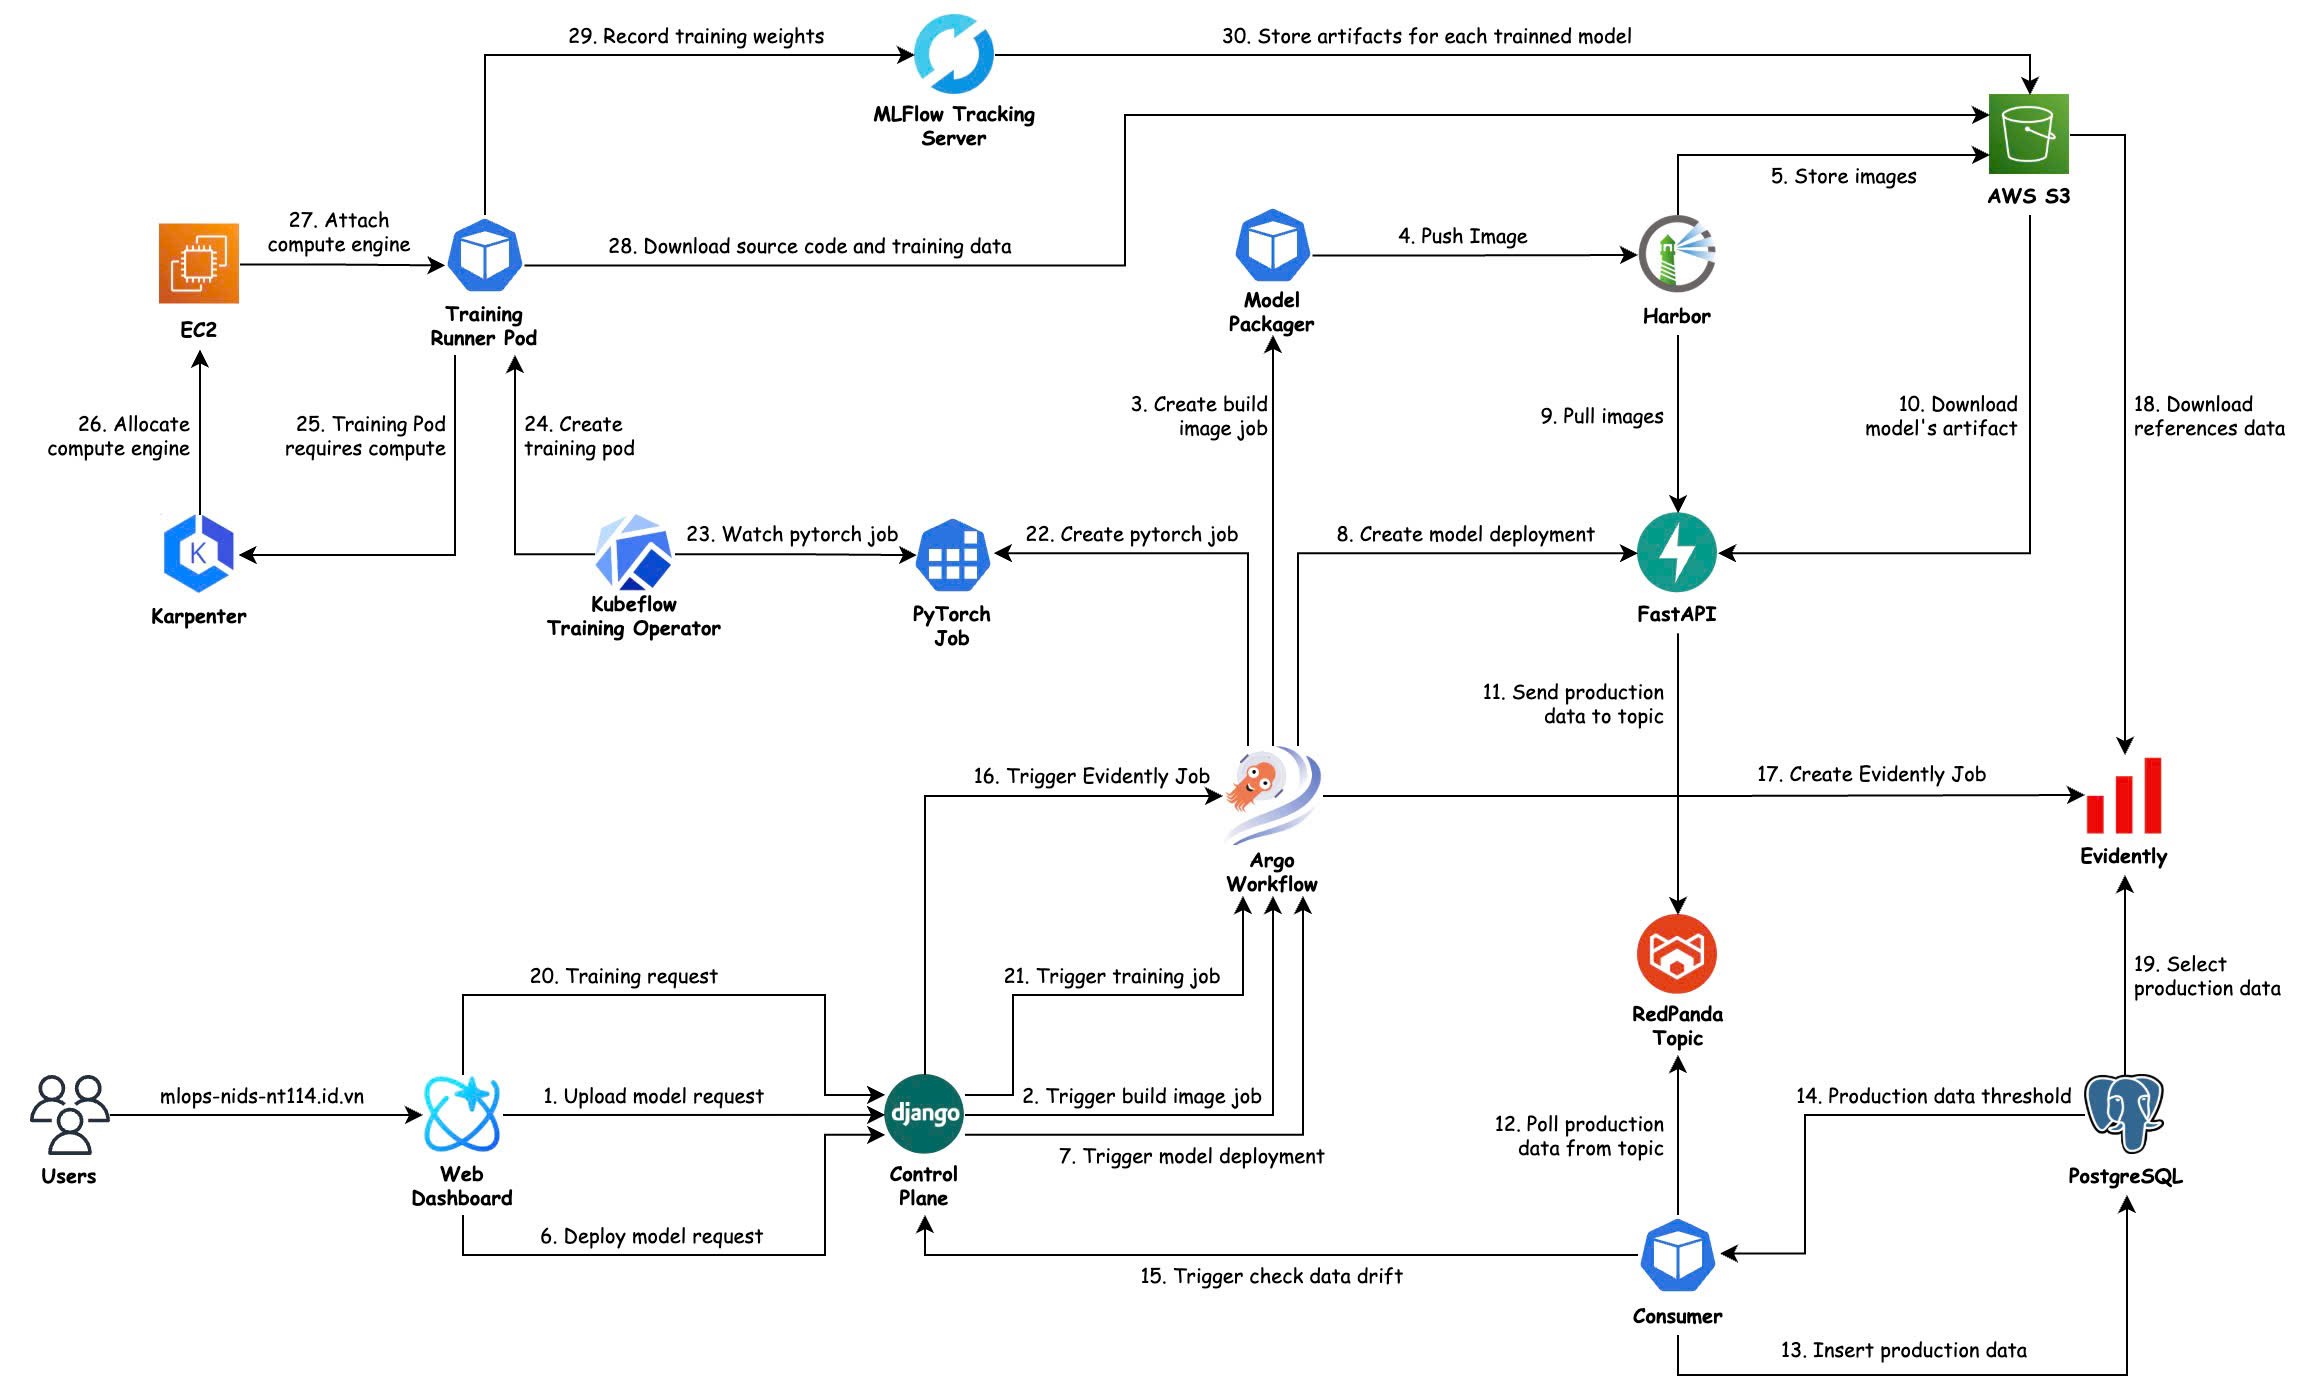
\includegraphics[width=0.8\linewidth]{assets/flow.png}
\caption{Configured prototype/testbed workflow. The Django control plane owns registry and lifecycle metadata; the FastAPI data plane handles serving and log emission. Argo/Kubeflow, object storage, Harbor, MLflow, Evidently, and Karpenter-backed compute are supporting adapters where configured.}
\label{fig:prototype-flow}
\end{figure}


\begin{table}[htbp]
\caption{Prototype modules, adapters, and configured responsibilities.}
\label{tab:implementation}
\centering
\small
\begin{tabular}{@{}L{2.6cm}L{2.8cm}L{6.0cm}@{}}
\toprule
\textbf{Module} & \textbf{Implementation} & \textbf{Responsibility} \\
\midrule
Control plane & Django/DRF & Records tenants, jobs, registry, deployment, and drift state. \\
Training execution & Argo/Kubeflow + runner & Configures entry-point execution and artifact return. \\
Artifact/registry layer & Object storage + PostgreSQL & Stores artifacts; owns product metadata and version state. \\
Packaging/serving & Packager + FastAPI & Configures artifact preparation, loading, and endpoint paths. \\
Logging/drift & Redpanda + consumer + Evidently & Configures log persistence and drift summaries. \\
Deployment configuration & Docker Compose/K8s/Argo files & Supports local integration and prototype/testbed deployment. \\
\bottomrule
\end{tabular}
\end{table}

\textit{Training execution.} In the configured Kubernetes path, the control plane submits a training webhook to Argo Events, and Argo Workflows may instantiate a Kubeflow \texttt{PyTorchJob} on Karpenter-backed nodes where configured. The runner path executes the selected entry point, exchanges \texttt{model.tar.gz} through S3-compatible storage, and returns completion metadata. User scripts need not import MLflow; optional tracking metadata does not determine Native Registry validity.

\textit{Metadata and registry.} On job-artifact ingestion, the control plane records available metrics, parameters, insights, and deployability summaries. The Native Registry groups family and version records linked to \texttt{ModelAPI} records, with PostgreSQL remaining the product-level source of truth for tenant ownership, lifecycle, and drift results. MLflow, when configured, provides internal tracking or serving adaptation rather than product-state ownership.

\textit{Packaging, serving, and monitoring.} The configured packaging path can build an image through Argo/Docker, push it to Harbor, and request a FastAPI pod; Section~8 does not evaluate each branch. In the prototype flow, prediction logs pass asynchronously through Redpanda to PostgreSQL, and Evidently produces monitoring reports. Drift remains a review signal, not an automatic redeployment decision.

\textit{Deployment and operational scope.} The submitted testbed configuration includes Docker Compose, Kubernetes (K3s) manifests, and Argo templates. Node provisioning through Karpenter is configured but its elasticity is not evaluated. The evidence exercises a controlled offline evaluation and one bounded serving replay; autonomous promotion, canary deployment, and production hardening remain future work.

Figures~\ref{fig:ui-evolution} and~\ref{fig:ui-drift} provide interface evidence for recorded registry state and an illustrative monitoring report.
\begin{figure}[htbp]
\centering
\begin{minipage}[t]{0.49\linewidth}
  \centering
  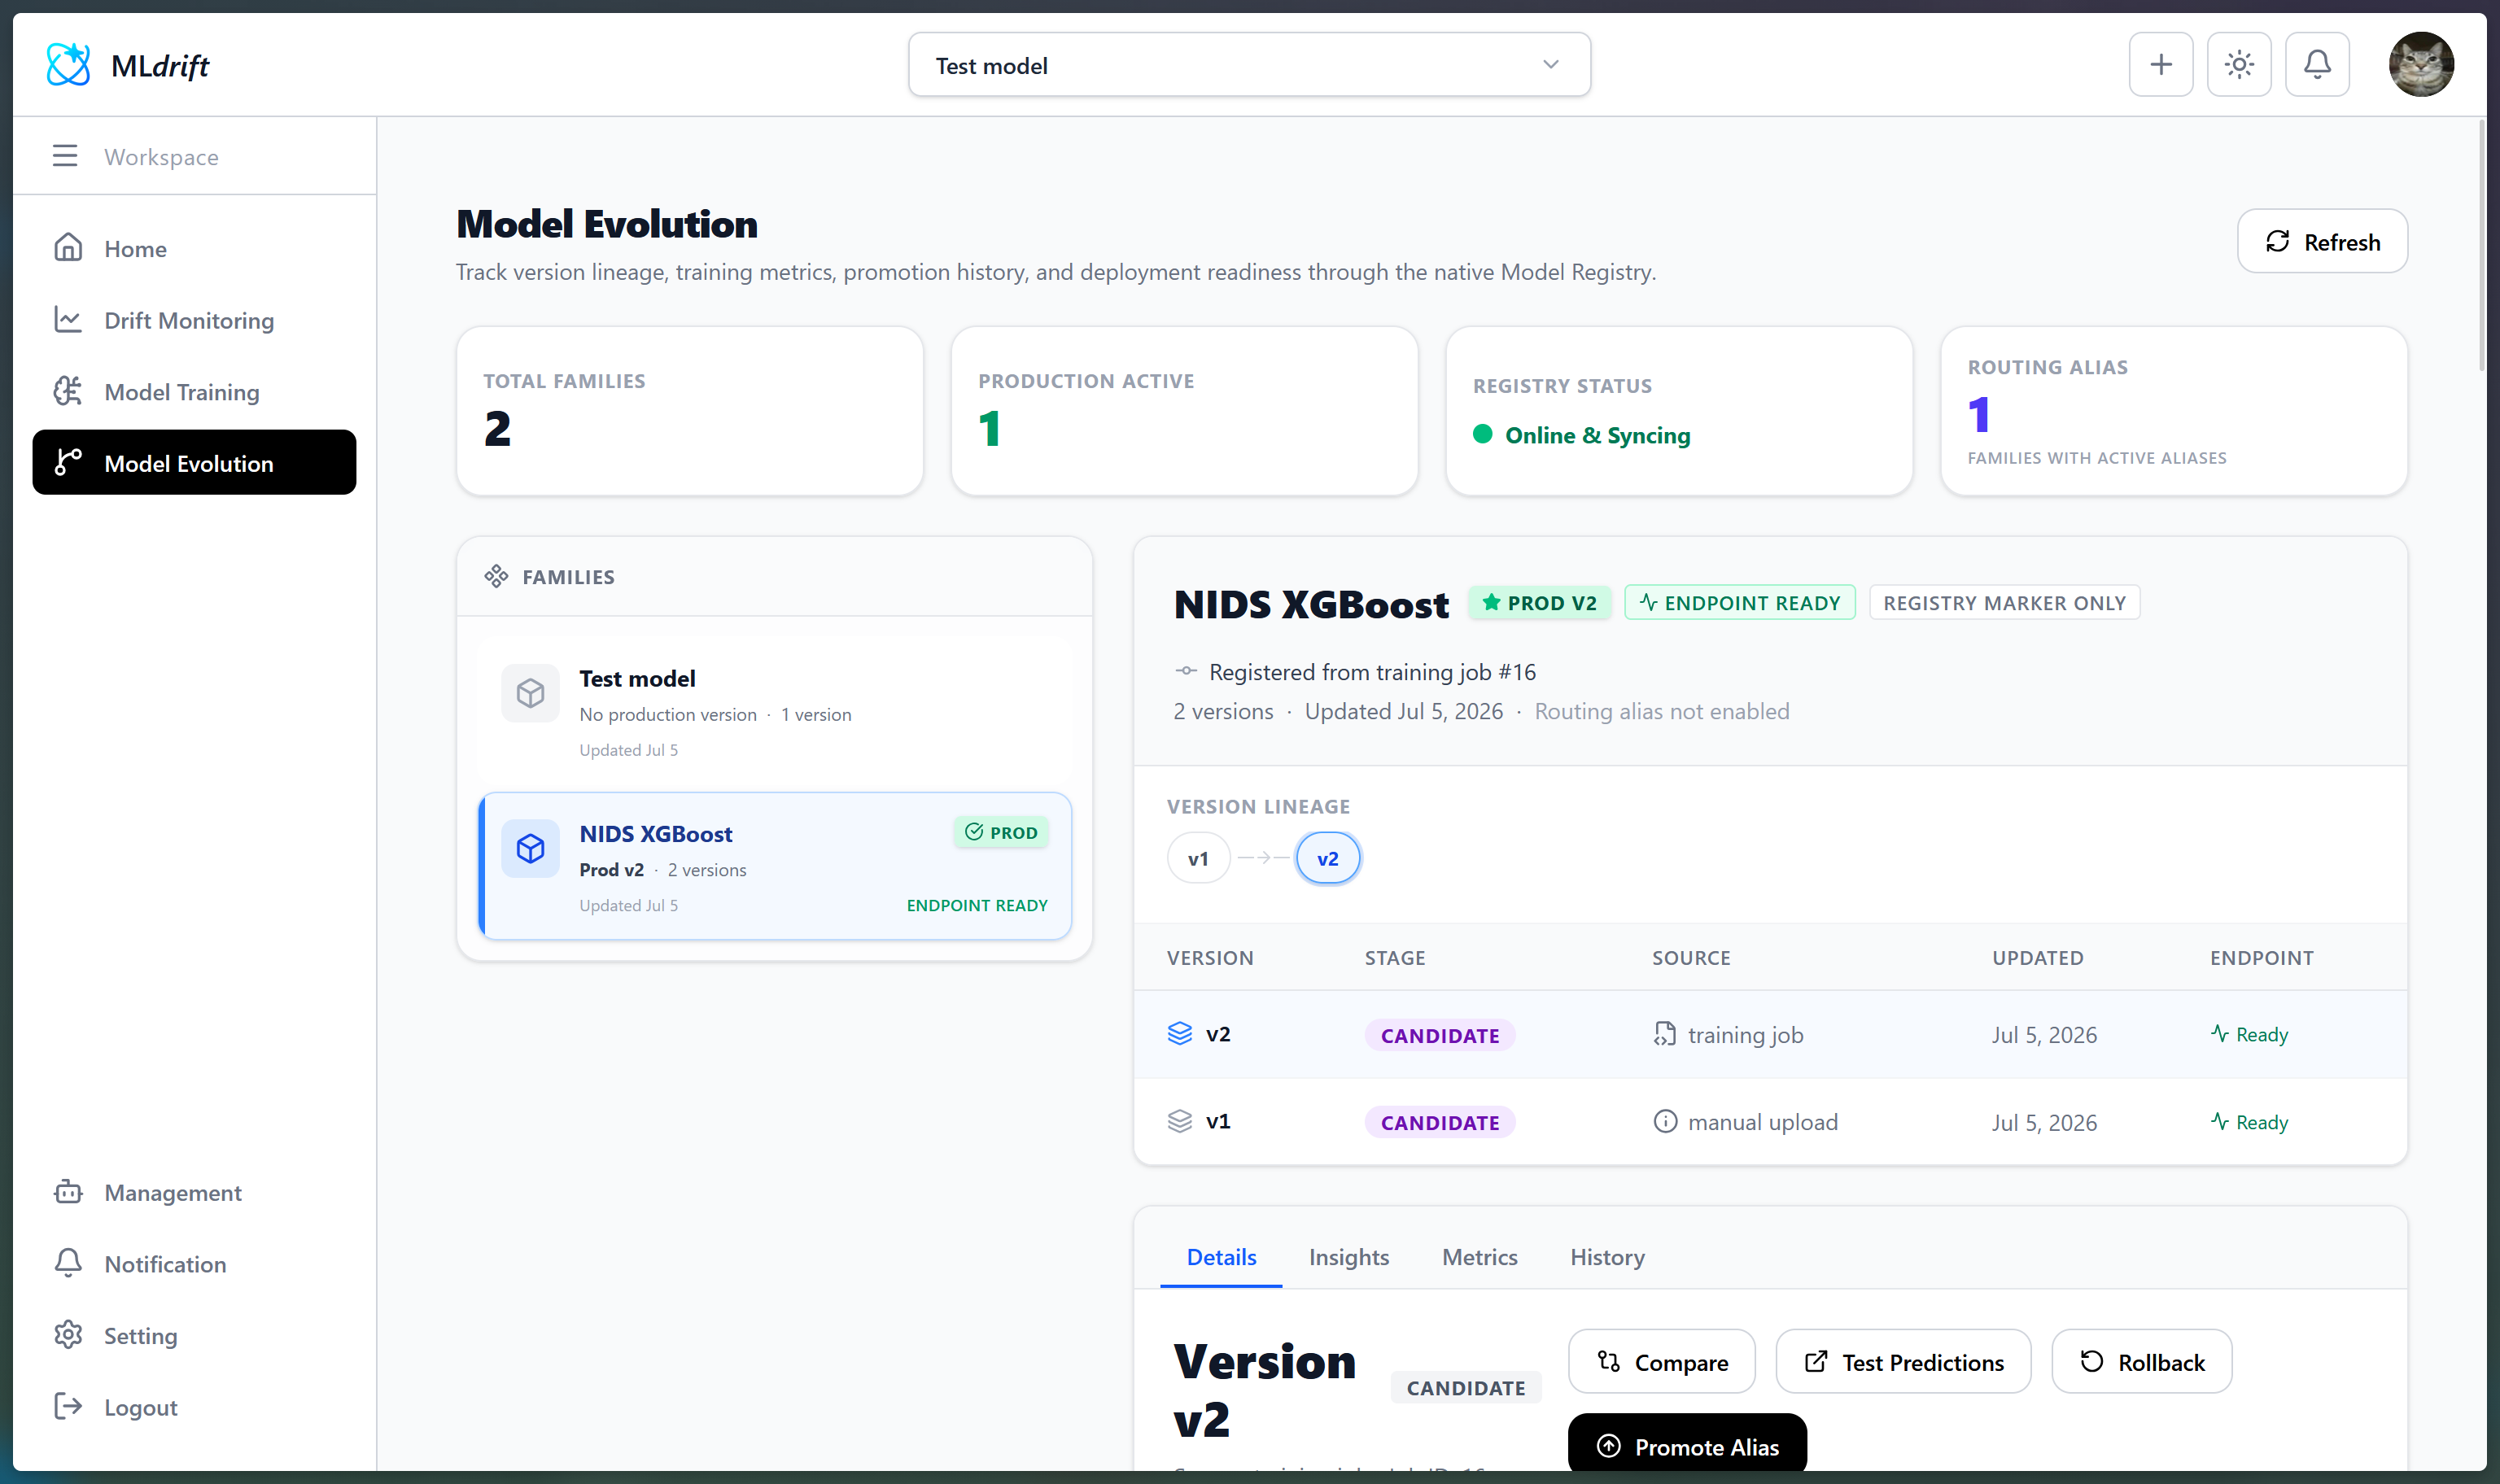
\includegraphics[width=\linewidth]{screenshots/10_model_evolution_v1_v2_lineage.png}
  \caption{Model Evolution UI recording v1--v2 lineage and registry-recorded serving-readiness metadata.}
  \label{fig:ui-evolution}
\end{minipage}\hfill
\begin{minipage}[t]{0.49\linewidth}
  \centering
  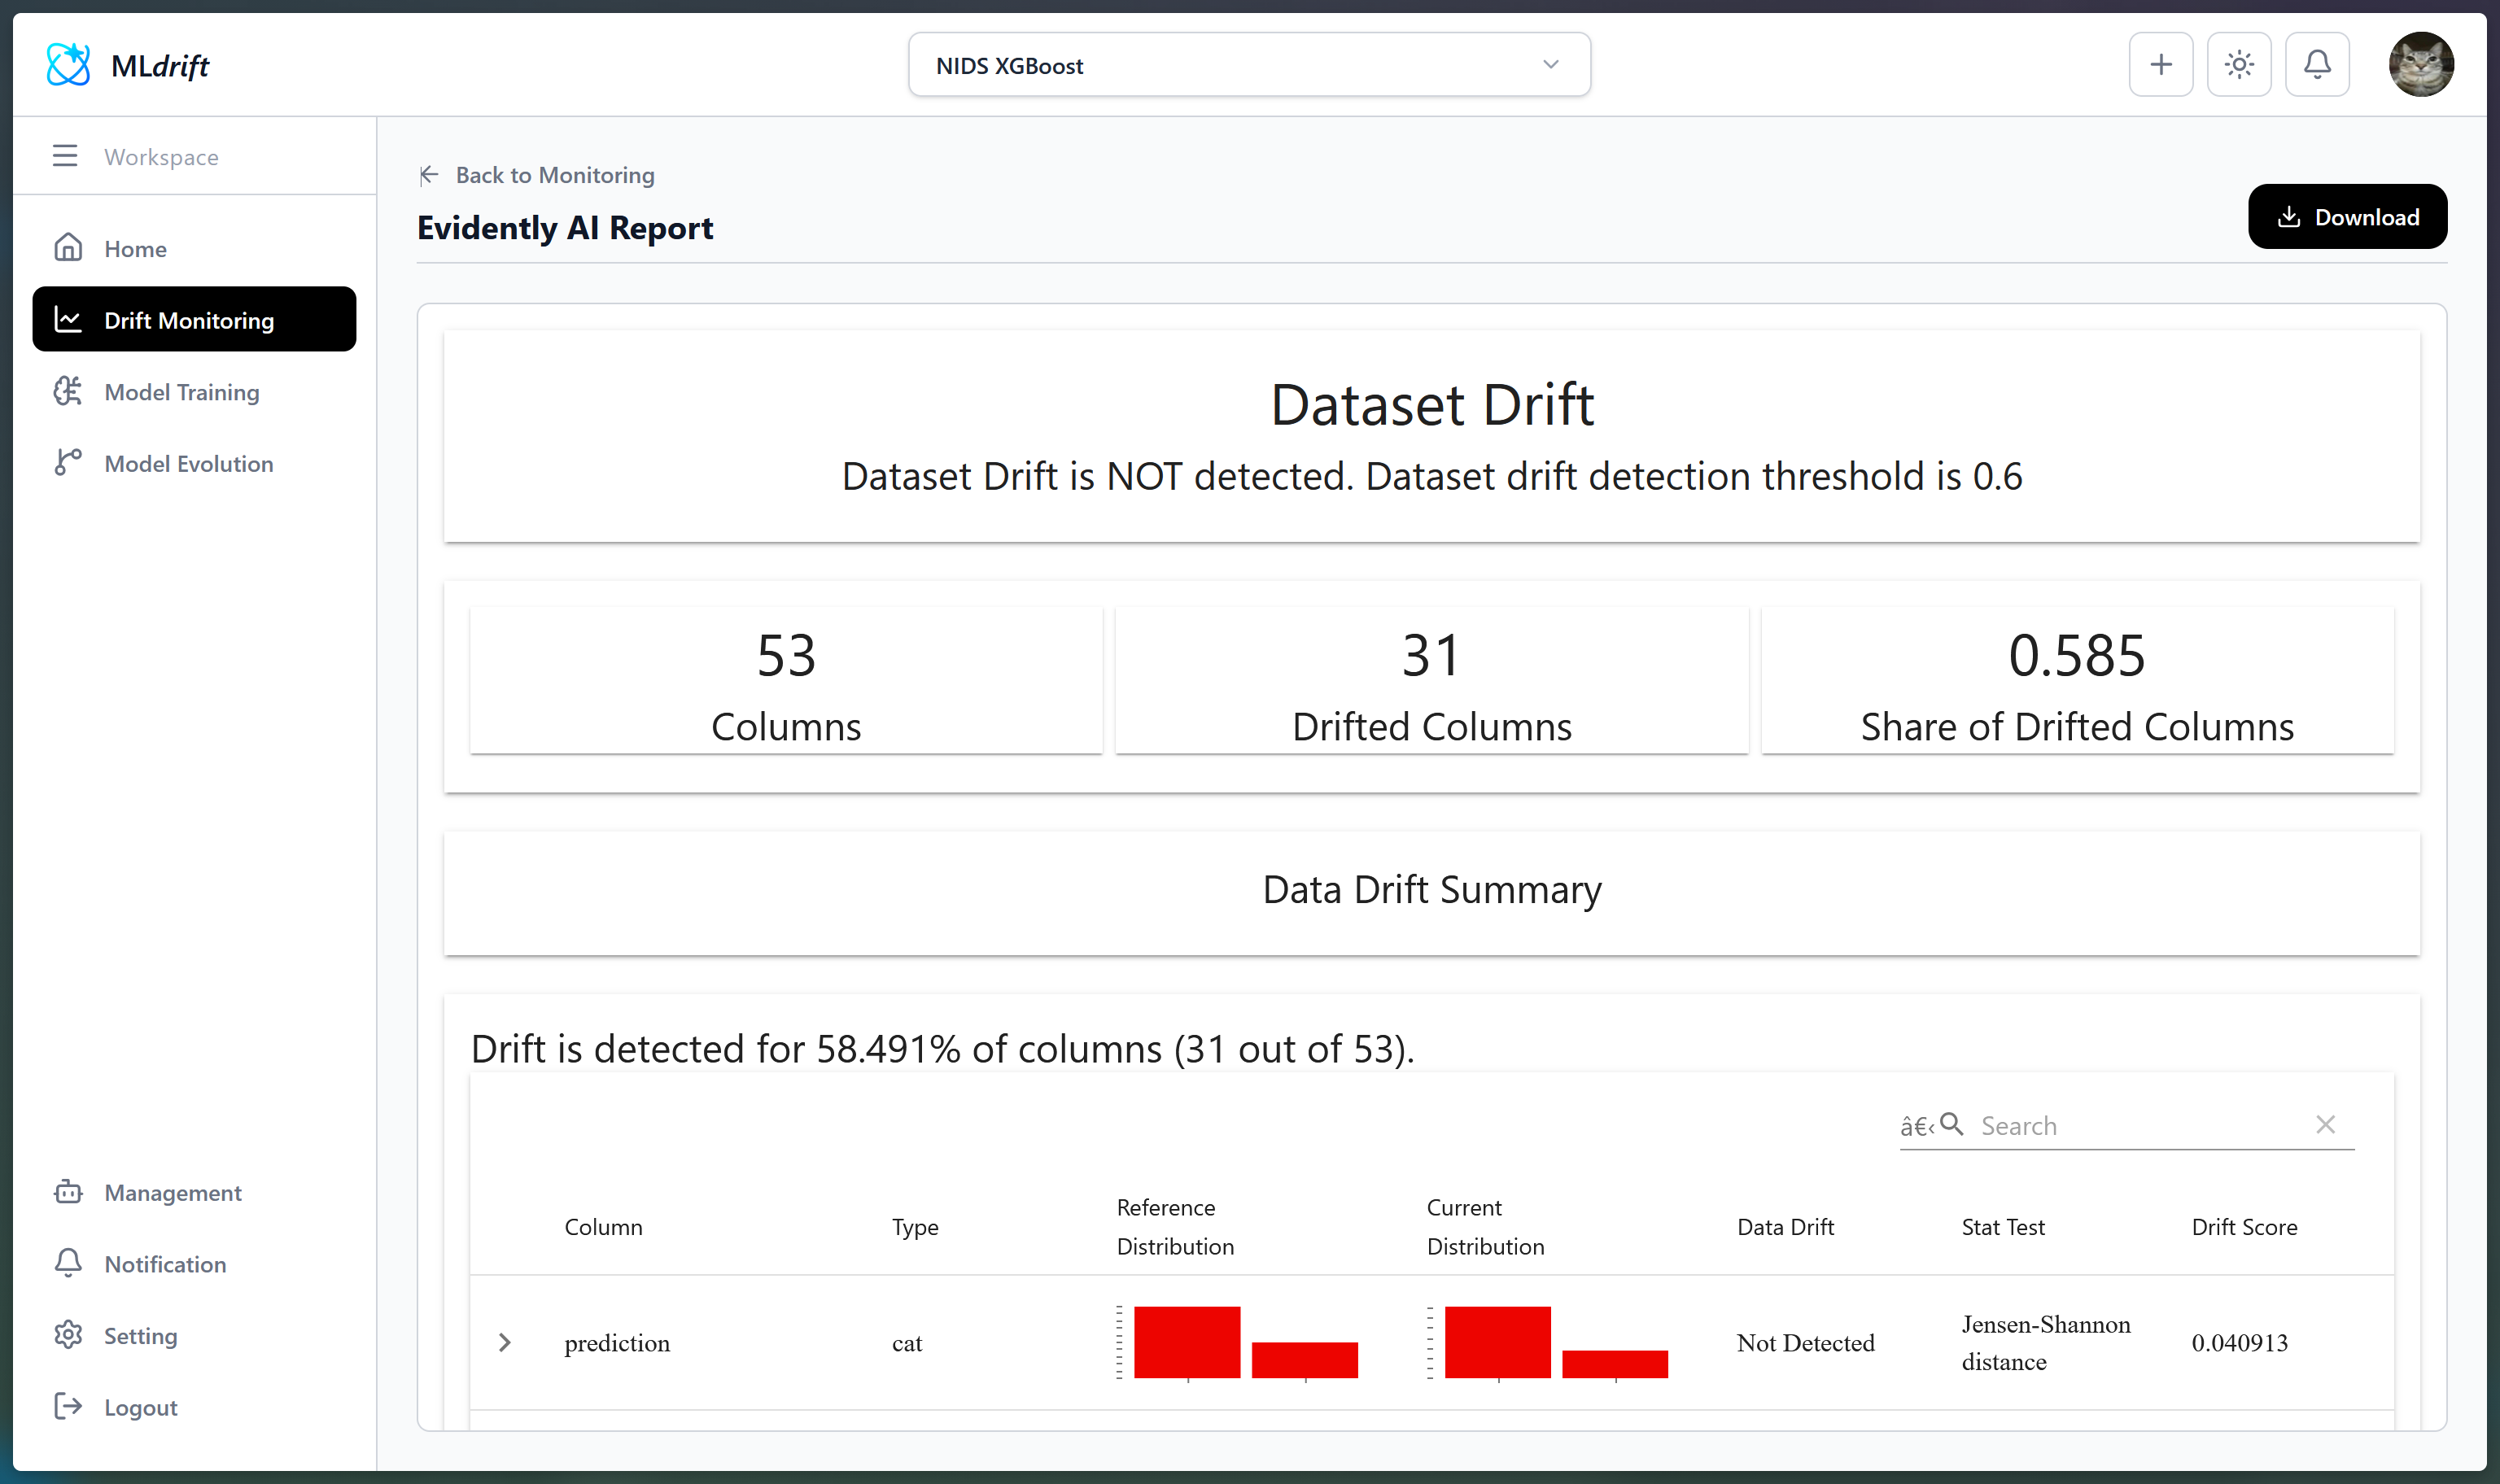
\includegraphics[width=\linewidth]{screenshots/14_drift_evidently_report_results.png}
  \caption{Illustrative drift-report UI. This standalone prototype run is independent of the nine controlled experimental windows reported in Table~\ref{tab:drift-multilevel}.}
  \label{fig:ui-drift}
\end{minipage}
\end{figure}

\FloatBarrier
\section{Preliminary Evaluation}

Evaluation focuses on feasibility under controlled splits, not NIDS optimization. The evaluator reads local tables \texttt{train\_2\_classes.csv}, \texttt{reference\_data.csv}, and three attack-family drift tables, referred to here as CIC-IDS2017-style data because the stored artifacts do not document their complete derivation from the original release. Each table provides 52 numeric flow features plus \texttt{Label}; non-BENIGN labels map to ATTACK, nonnumeric values are coerced, and missing or infinite values are imputed with medians from the fixed-model training sample. The fixed XGBoost model uses at most 100,000 sampled training rows after exact future-ATTACK row hashes are removed.

Each attack table is shuffled and split into 60\% trigger/retraining and 40\% future-holdout pools. Trigger/future counts are 30,000 and 20,000 for PortScan, 4,890 and 3,260 for BruteForce, and 1,029 and 686 for WebAttacks. A per-family challenger uses the cleaned fixed-model training rows plus its trigger ATTACK rows. $D_{\mathrm{ref}}$ consists of the BENIGN rows in a 50,000-row sample of \texttt{reference\_data.csv}; held-out windows combine up to 5,000 future ATTACK rows with BENIGN rows from that same pool at three controlled attack fractions: Mild ($\approx$15\%), Moderate ($\approx$40\%), and Severe ($\approx$85\%). BENIGN rows are therefore not disjoint between $D_{\mathrm{ref}}$ and the controlled windows. Hashing numeric features plus normalized labels removes exact future-ATTACK duplicates from model fitting; it does not exclude session-, capture-, preprocessing-, correlated-flow-, or semantic overlap.

For each of 52 features, a two-sided KS test sets $I_j=1$ at uncorrected $p_j<\alpha=0.05$; the dataset rule is $\rho\geq\tau_D$ with $\tau_D=0.30$. As a post-hoc check, both Bonferroni ($\alpha/52\approx9.6\times10^{-4}$) and Benjamini--Hochberg corrections were applied: the most conservative case (Bonferroni, WebAttacks Mild) reduces the drifted count from 51 to 43 of 52 ($\rho=0.83$), which still exceeds $\tau_D$; all other scenarios retain 50--51 drifted features. No drift decision changes under either correction. The reported mean KS is the mean test statistic and is descriptive, not the alert rule. The experiment is repeated over five random seeds (42, 123, 456, 789, 1024); Table~\ref{tab:drift-multilevel} reports the mean values.


\begin{table}[htbp]
\centering
\caption{Controlled challenger evaluation (mean$\pm$std over 5 seeds). Mean KS is descriptive across 52 features; $\Delta$M-F1 is computed before display rounding.}
\label{tab:drift-multilevel}
\scriptsize
\setlength{\tabcolsep}{3pt}
\begin{tabular}{@{}llccccc@{}}
\toprule
Attack Family & Level & Atk\% & Mean KS & Fixed M-F1 & Chall. M-F1 & $\Delta$M-F1 \\
\midrule
\multirow{3}{*}{PortScan}
  & Mild     & 17\% & 0.101$\pm$0.001 & 0.453$\pm$0.000 & 0.999$\pm$0.000 & +0.547 \\
  & Moderate & 40\% & 0.233$\pm$0.001 & 0.375$\pm$0.000 & 1.000$\pm$0.000 & +0.625 \\
  & Severe   & 85\% & 0.496$\pm$0.001 & 0.130$\pm$0.000 & 1.000$\pm$0.000 & +0.869 \\
\midrule
\multirow{3}{*}{BruteForce}
  & Mild     & 15\% & 0.068$\pm$0.001 & 0.461$\pm$0.001 & 1.000$\pm$0.000 & +0.539 \\
  & Moderate & 40\% & 0.182$\pm$0.002 & 0.376$\pm$0.001 & 1.000$\pm$0.000 & +0.623 \\
  & Severe   & 85\% & 0.385$\pm$0.004 & 0.132$\pm$0.001 & 0.998$\pm$0.001 & +0.867 \\
\midrule
\multirow{3}{*}{WebAttacks}
  & Mild     & 15\% & 0.085$\pm$0.001 & 0.459$\pm$0.000 & 0.998$\pm$0.000 & +0.538 \\
  & Moderate & 40\% & 0.228$\pm$0.001 & 0.375$\pm$0.000 & 0.997$\pm$0.001 & +0.622 \\
  & Severe   & 85\% & 0.480$\pm$0.003 & 0.130$\pm$0.000 & 0.988$\pm$0.003 & +0.857 \\
\bottomrule
\end{tabular}
\end{table}

All nine windows satisfy the $0.30$ dataset rule, with 50--51 of 52 features marked drifted. As the controlled attack fraction rises, mean KS increases from 0.07--0.10 to 0.38--0.50 and fixed-model Macro-F1 falls from about 0.46 to 0.13. The corresponding challengers achieve Macro-F1 of 0.988--1.000. Over five seeds, standard deviations remain below 0.004 for all reported metrics, indicating that the results are stable with respect to random sampling. Because trigger and future-holdout rows share the same source distribution (i.i.d.\ split) and CIC-IDS2017 attack classes are well separated in the 52-feature space, the near-perfect challenger scores reflect the constructed evaluation setting rather than general robustness. The primary signal is the recovery gap $\Delta$M-F1: the framework detects drift and the retrained challenger recovers Macro-F1 by 0.54--0.87 depending on severity. These results demonstrate lifecycle feasibility in this controlled setting, not robustness across environments, natural drift, or general adaptation effectiveness.

One bounded testbed replay used 100 Locust users for approximately 89 seconds and issued 4,343 client-side requests. Locust recorded 47.6 requests/s on average, 1.74 s mean response time, 2.30 s p95, and four HTTP 502 responses. Prometheus recorded a 144.1 requests/s peak server-side rate and 1.60 s mean handler latency. Client averages and server-side peaks use different measurement and aggregation semantics and are not directly comparable. This single observation is not capacity, scalability, reliability, availability, SLA, or production evidence. Figure~\ref{fig:endpoint-benchmark} shows the client-side time series.

\begin{figure}[t]
\centering
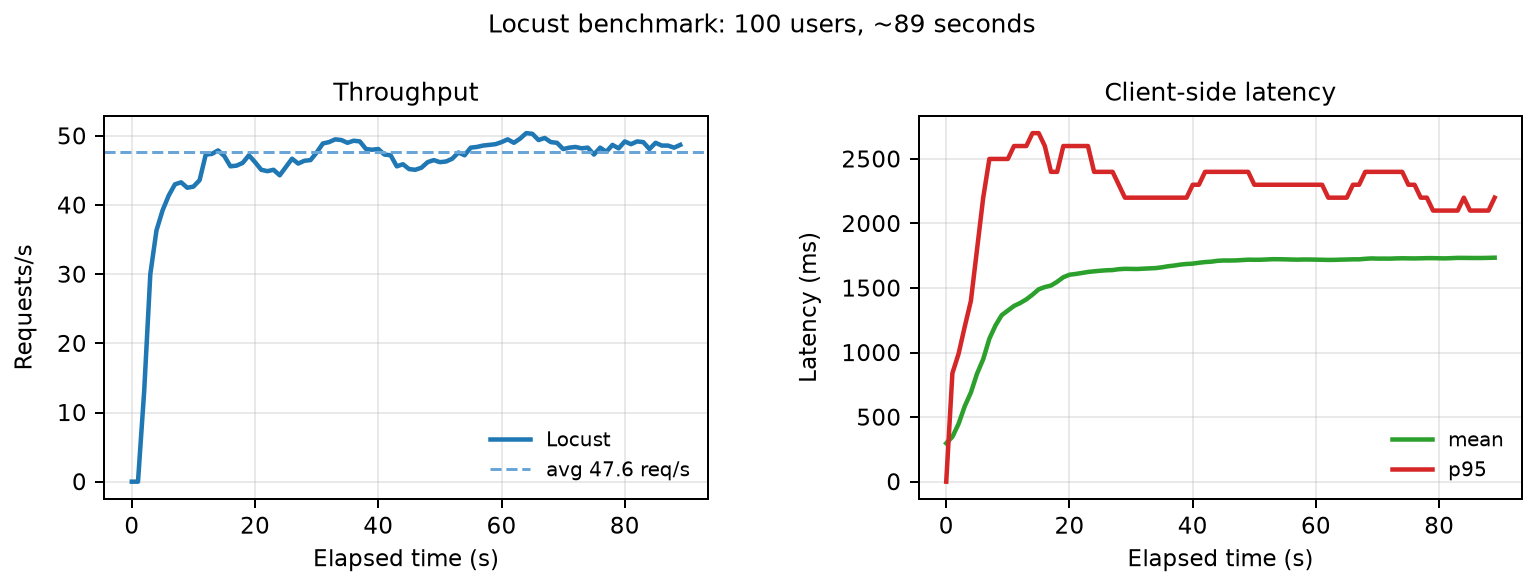
\includegraphics[width=0.8\linewidth]{assets/chart-locust-benchmark.png}
\caption{One bounded testbed replay: 100 Locust users over an $\approx$89-second window.}
\label{fig:endpoint-benchmark}
\end{figure}

\section{Discussion}

The framework treats monitoring reports as control-plane lifecycle evidence. The Native Registry matters as the tenant-facing owner of model-version, deployability, log-summary, drift-result, and review state while serving and monitoring remain replaceable adapters.

The scope is intentionally limited. First, the system targets tabular classification artifacts; image, text, time-series, and large language models need additional schema validation and monitoring metrics. Second, arbitrary user-uploaded artifacts introduce security risks, so hardened systems must isolate execution, validate dependencies, restrict archive extraction, and enforce resource quotas. Third, autonomous retraining and promotion require reliable evaluation gates, rollback policies, and human approval. Therefore, this baseline treats drift detection as an adaptation signal rather than an unconditional redeployment decision.

\section{Conclusion}

This paper presented a baseline drift-aware MLOps framework with a tenant-aware control-plane/data-plane architecture, a drift-aware lifecycle formulation, and preliminary NIDS case-study evidence. Its PostgreSQL-backed Native Registry remains the product-level source of truth for ownership, versions, deployability metadata, log summaries, drift results, and lifecycle state; MLflow and other tools are adapters where configured. One controlled challenger run and one bounded testbed replay support prototype feasibility, not general effectiveness or production-scale validation. NIDS remains a case study, and retraining, promotion, or rollback require human review rather than autonomous lifecycle management.

\begin{thebibliography}{00}

\bibitem{kreuzberger2023mlops}
M. Kreuzberger, N. Kuhl, and S. Hirschl, ``Machine Learning Operations (MLOps): Overview, Definition, and Architecture,'' \textit{IEEE Access}, vol. 11, pp. 31866--31879, 2023.

\bibitem{sculley2015debt}
D. Sculley, G. Holt, D. Golovin, E. Davydov, T. Phillips, D. Ebner,
V. Chaudhary, M. Young, J.-F. Crespo, and D. Dennison,
``Hidden Technical Debt in Machine Learning Systems,''
in \textit{Advances in Neural Information Processing Systems}, vol. 28, 2015.

\bibitem{amershi2019software}
S. Amershi, A. Begel, C. Bird, R. DeLine, H. Gall, E. Kamar,
N. Nagappan, B. Nushi, and T. Zimmermann,
``Software Engineering for Machine Learning: A Case Study,''
in \textit{Proc. IEEE/ACM 41st International Conference on Software Engineering:
Software Engineering in Practice}, 2019, pp. 291--300.

\bibitem{john2021towards}
M. M. John, H. H. Olsson, and J. Bosch, ``Towards MLOps: A Framework and Maturity Model,'' in \textit{Proc. 47th Euromicro Conference on Software Engineering and Advanced Applications}, 2021, pp. 1--8.

\bibitem{zhou2020pipeline}
Y. Zhou, Y. Yu, and B. Ding, ``Towards MLOps: A Case Study of ML Pipeline Platform,'' in \textit{Proc. International Conference on Artificial Intelligence and Computer Engineering}, 2020, pp. 494--500.

\bibitem{baylor2017tfx}
D. Baylor et al.,
``TFX: A TensorFlow-Based Production-Scale Machine Learning Platform,''
in \textit{Proc. 23rd ACM SIGKDD International Conference on Knowledge Discovery and Data Mining},
2017, pp. 1387--1395.

\bibitem{subramanya2022devops}
S. G. Subramanya, S. Shetty, V. Patil, S. K. Gad, and S. N. Bhat, ``From DevOps to MLOps: Overview and Application to Electricity Market Forecasting,'' \textit{Applied Sciences}, vol. 12, no. 19, 2022.

\bibitem{renggli2021data}
C. Renggli, B. Karlaš, B. Ding, F. Liu, K. Schawinski, W. Wu, and C. Zhang, ``A Data Quality-Driven View of MLOps,'' \textit{arXiv preprint arXiv:2102.07750}, 2021.

\bibitem{polyzotis2017data}
N. Polyzotis, S. Roy, S. E. Whang, and M. Zinkevich,
``Data Management Challenges in Production Machine Learning,''
in \textit{Proc. ACM International Conference on Management of Data}, 2017,
pp. 1723--1726.

\bibitem{gama2014survey}
J. Gama, I. Zliobaite, A. Bifet, M. Pechenizkiy, and A. Bouchachia, ``A Survey on Concept Drift Adaptation,'' \textit{ACM Computing Surveys}, vol. 46, no. 4, pp. 1--37, 2014.

\bibitem{webb2016drift}
G. I. Webb, R. Hyde, H. Cao, H.-L. Nguyen, and F. Petitjean,
``Characterizing Concept Drift,''
\textit{Data Mining and Knowledge Discovery}, vol. 30, no. 4,
pp. 964--994, 2016.

\bibitem{mlflow}
M. Zaharia et al., ``Accelerating the Machine Learning Lifecycle with MLflow,'' \textit{IEEE Data Engineering Bulletin}, vol. 41, no. 4, pp. 39--45, 2018.

\bibitem{crankshaw2017clipper}
D. Crankshaw, X. Wang, G. Zhou, M. J. Franklin, J. E. Gonzalez, and I. Stoica,
``Clipper: A Low-Latency Online Prediction Serving System,''
in \textit{Proc. 14th USENIX Symposium on Networked Systems Design and Implementation},
2017, pp. 613--627.

\bibitem{xgboost}
T. Chen and C. Guestrin, ``XGBoost: A Scalable Tree Boosting System,'' in \textit{Proc. 22nd ACM SIGKDD International Conference on Knowledge Discovery and Data Mining}, 2016, pp. 785--794.

\bibitem{cicids}
I. Sharafaldin, A. H. Lashkari, and A. A. Ghorbani, ``Toward Generating a New Intrusion Detection Dataset and Intrusion Traffic Characterization,'' in \textit{Proc. 4th International Conference on Information Systems Security and Privacy}, 2018, pp. 108--116.

\bibitem{sommer2010closedworld}
R. Sommer and V. Paxson,
``Outside the Closed World: On Using Machine Learning for Network Intrusion Detection,''
in \textit{Proc. IEEE Symposium on Security and Privacy}, 2010, pp. 305--316.

\bibitem{kubernetes}
B. Burns, B. Grant, D. Oppenheimer, E. Brewer, and J. Wilkes, ``Borg, Omega, and Kubernetes,'' \textit{Communications of the ACM}, vol. 59, no. 5, pp. 50--57, 2016.

\bibitem{Bhatt2025HarmonE}
H. Bhatt, S. Biswas, S. Rakhunathan, and K. Vaidhyanathan,
``HarmonE: A Self-Adaptive Approach to Architecting Sustainable MLOps,''
arXiv preprint arXiv:2505.13693, 2025. Accepted to ECSA 2025.
DOI: 10.48550/arXiv.2505.13693.

\bibitem{Zhang2025SSFNIDS}
X. Zhang, R. Zhao, Z. Jiang, H. Chen, Y. Ding, E. C. H. Ngai, and S.-H. Yang,
``Continual Learning with Strategic Selection and Forgetting for Network Intrusion Detection,''
arXiv preprint arXiv:2412.16264, 2025. Accepted by IEEE INFOCOM 2025.
DOI: 10.48550/arXiv.2412.16264.

\bibitem{MarcosMercade2026MLOpsFrameworks}
J. Marcos-Mercad\'e, U. Lopez-Novoa, and M. Ega\~na Aranguren,
``An Empirical Evaluation of Modern MLOps Frameworks,''
arXiv preprint arXiv:2601.20415, 2026.

\end{thebibliography}

\end{document}
